\documentclass [PhD] {UCLAthesis}
\graphicspath{ {figures/} }
\usepackage{overpic}
\usepackage{array}
\usepackage{makecell}
\usepackage{pifont}
\usepackage{algorithm, algpseudocode}
\usepackage{lipsum}
\usepackage{float}
\usepackage[letterpaper, left=1.1in, right=1.1in, top=1.1in, bottom=1.1in]{geometry}


\newcommand{\cmark}{\ding{51}}%
\newcommand{\xmark}{\ding{55}}%
\algnewcommand{\IfThenElse}[3]{% \IfThenElse{<if>}{<then>}{<else>}
  \State \algorithmicif\ #1\ \algorithmicthen\ #2\ \algorithmicelse\ #3}

\title          {A real sick dissertation}
\author         {Bill Withers}
\department     {Neuroscience}
\degreeyear     {2024}
%
\chair{A\$AP Rocky}
\member{A\$AP Yams}
\member{A\$AP Twelvyy}
\member{A\$AP Nast}
%
\dedication{\textsl{ 
            \textit{Non enim tranquillis maribus naucleri periti fiunt}
            }}
%

\acknowledgments { 

\textbf{First, I acknowledge and thank my haters:}
In fourth grade, there was a day when the entire class was eager to play basketball during recess. As the only one who brought a ball, I made sure everyone had a chance to join the game, passing the ball around and encouraging teamwork. However, one hater, James Roberts, told the teacher and other kids that I refused to share. I was bewildered and hurt, knowing that I had done my best to include everyone. Despite my frustration, I continued to offer the ball, hoping my actions would speak louder than James' words. This experience taught me the value of perseverance and integrity, driving me to excel academically and personally. Fueled by this motivation, I earned a PhD at UCLA to spite James who never gradutated high school. 

\\
\textbf{I acknowledge the funding sources that greatly contributed to my training as a scientist and made this research possible:}\\


\begin{itemize}
  \item \textbf{NIH T32XXXXX}
  \item \textbf{NIH F31XXXXX}
  \item \textbf{NIH U01XXXXX}
\end{itemize}
}

%

\vitaitem{2010--2014}{B.S. in Biology, UCLA}
\vitaitem{2016--2024}{Graduate Student Researcher in Neurology, UCLA}

%

\publication{\textbf{Madruga, B. A.}, Dorian, C. C., Sehgal, M., Silva, A. J., Shtrahman, M., Aharoni, D., \& Golshani, P.   Open-source, high performance miniature multiphoton microscopy systems for freely behaving animals. \textit{BioRxiv Preprint}, \textbf{2024}}



\abstract{
This dissertation is focused on things.}
  
\begin{document}

\makeintropages

\chapter{Introduction to Fluorescent Imaging and Microscopy in Neuroscience}\label{ch:Intro}
\section{A Brief History of Using Light to Study Nature}
Scientists have used optical systems to study nature for centuries, as these systems extend the capabilities of our native visual capacity as humans. From as early as 1608, scientists designed and used refractive telescopes to better visualize and record the complicated movements of planets and stars, thereby validating the heliocentric model of our solar system proposed by Copernicus \cite{Copernicus1543}. Cells, the principle units of life, were discovered by Robert Hooke (of spring constant fame) in 1665 in the text \textit{Micrographia}, using a microscope featuring a condenser lenses made of a brine-filled sphere\cite{Hooke1665}. Nearly two hundred years later, neuroscientists like Camillo Golgi and Santiago Ramón y Cajal used optical means in combination with chemical staining techniques to provide an optical contrast between neural cells and the surrounding tissue background \cite{Golgi1873, Cajal1899}. In doing so, these pioneering researchers studied and characterized many foundational structural aspects of the central and peripheral nervous system and used that understanding to make informed predictions as to how the circuitry may function in living systems. Today, researchers rely heavily on fluorescence microscopy systems in combination with genetic molecular tools to provide spectral contrast between neural populations of interest and the surrounding tissue, enabling the study of neurons in high spatial and temporal resolution. 

\section{Fluorescence as a Physical Process}\label{sec:fluorescence_physical}

\begin{figure*}
\centering
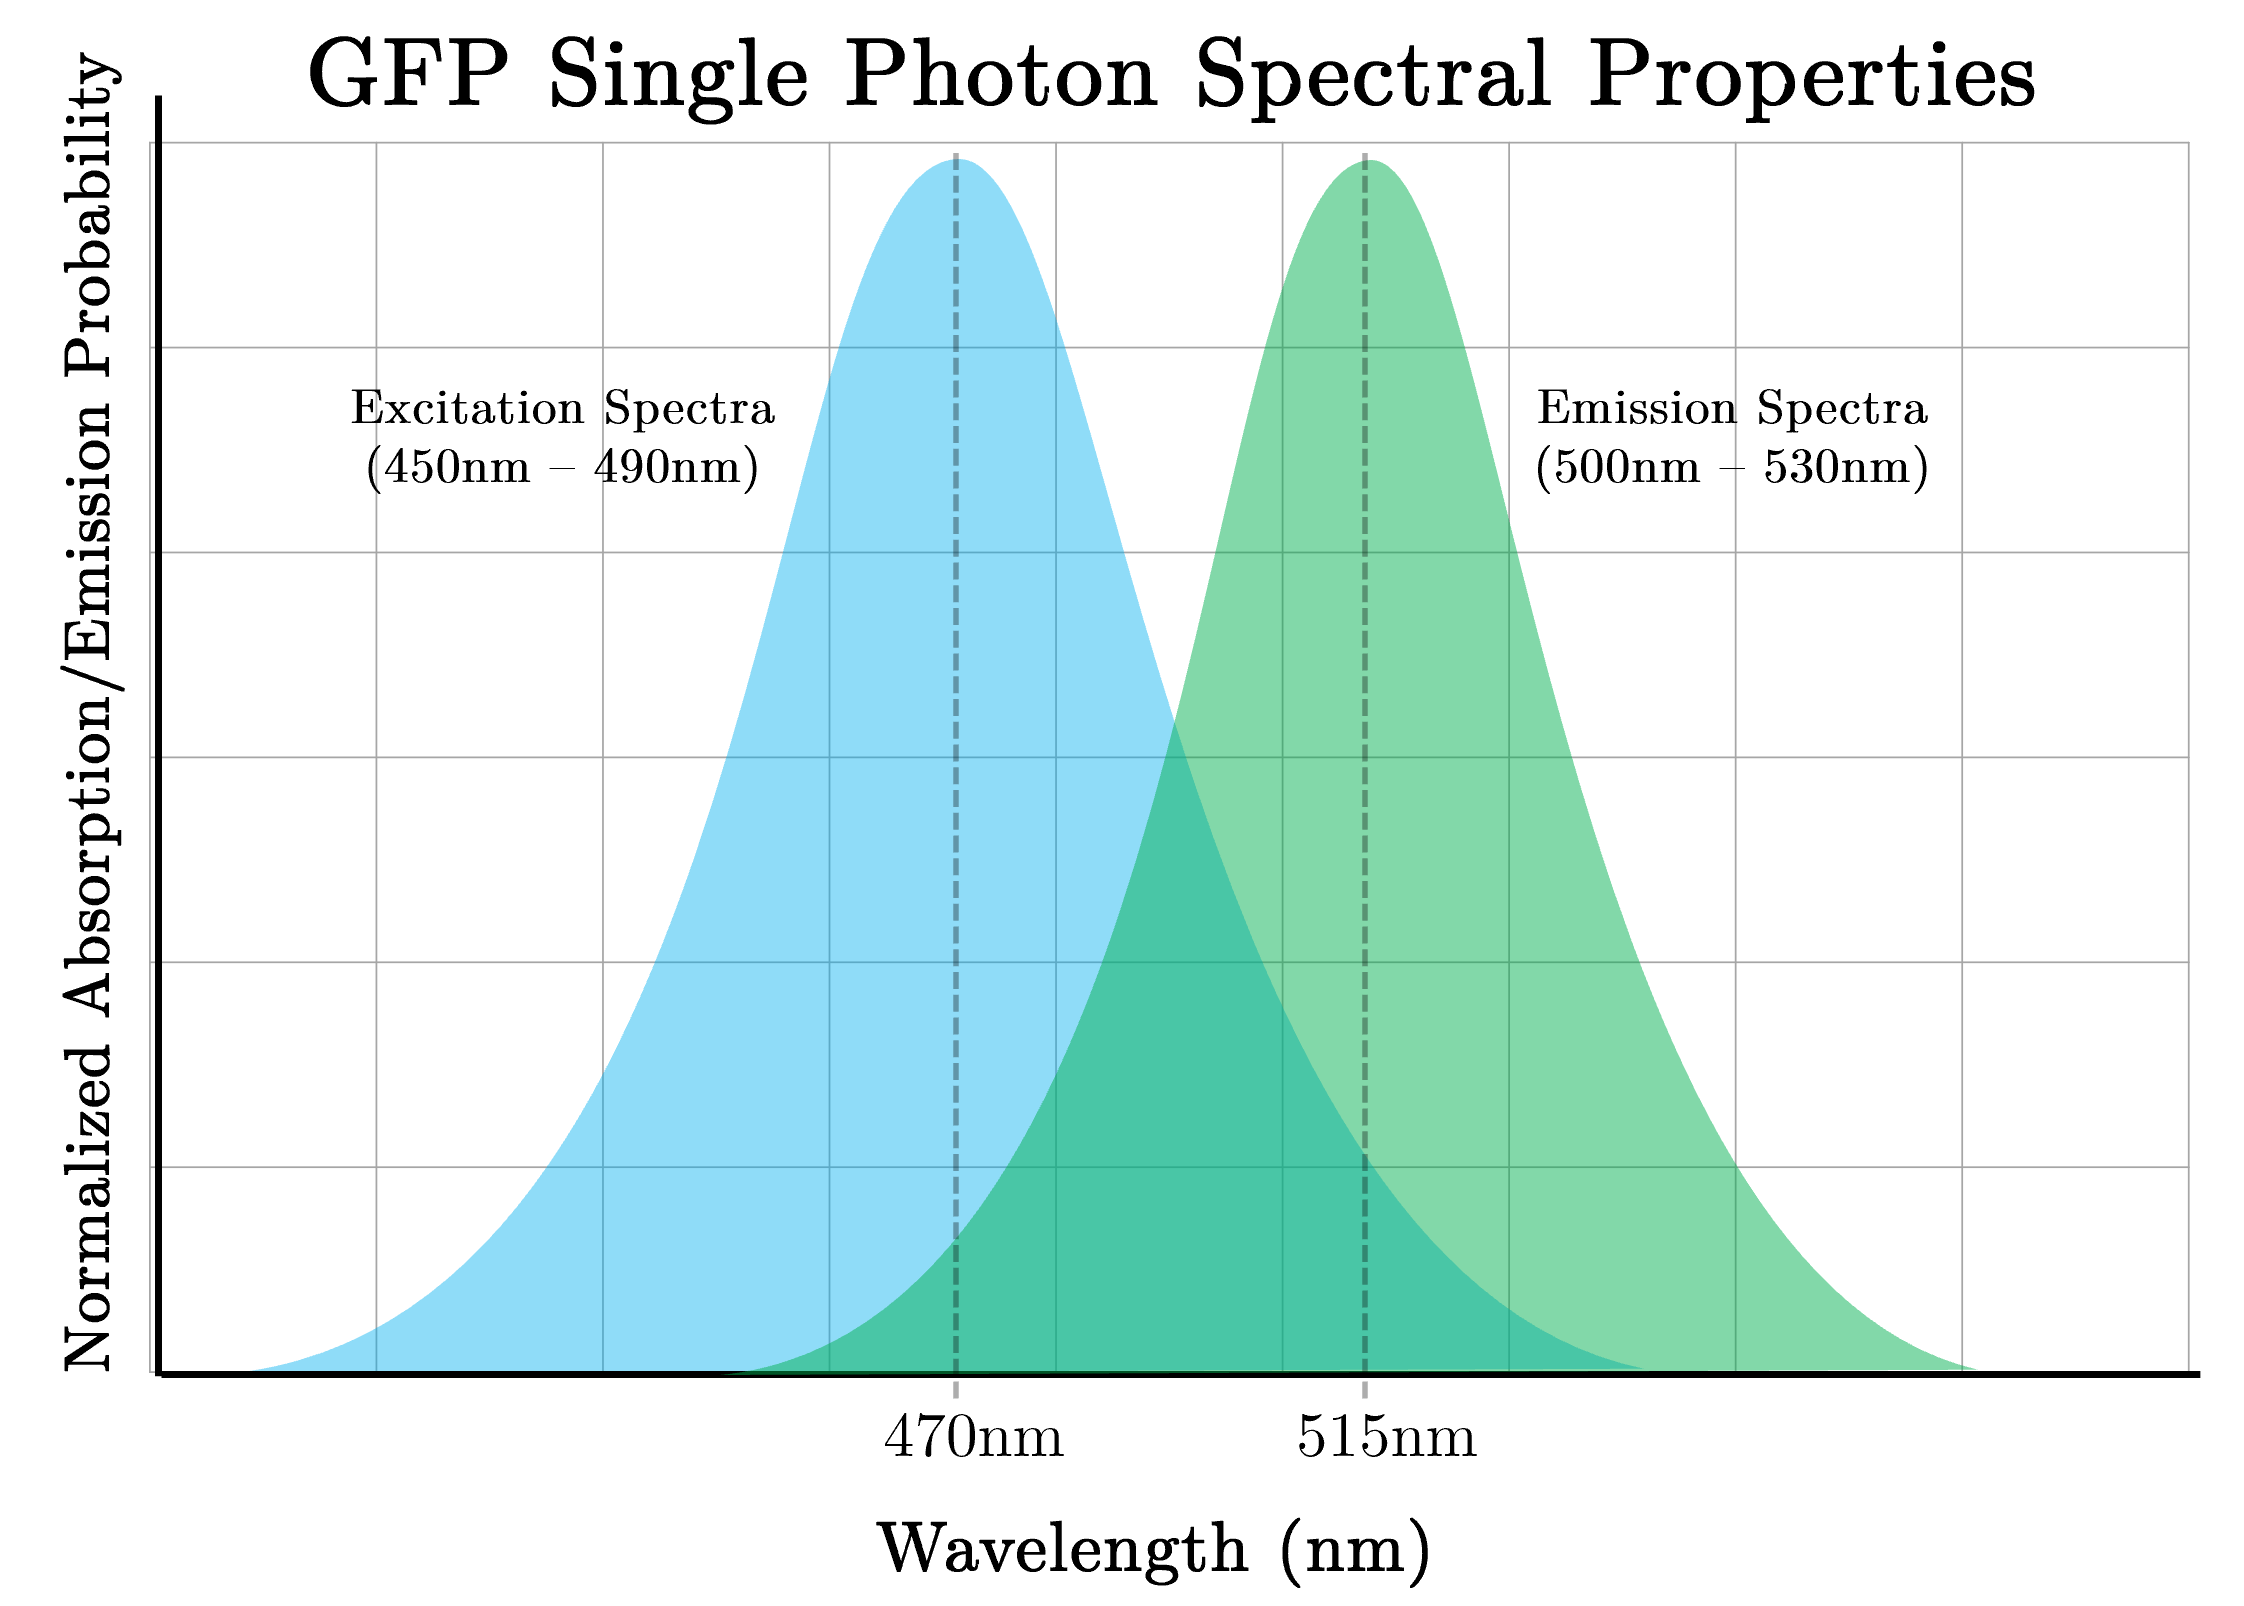
\includegraphics[width=0.9\linewidth]{Figures/GFP.PNG}
\caption{\textbf{Approximate Single Photon Spectral Properties of GFP}}
\raggedright
Green fluorescent protein is able to accept photons within the bandwidth shown under the blue curve, with the height denoting the likelihood with which the photon is absorbed. The green curve represents the emission bandwidth and the likelihood of an emitted photon taking a particular energy.
\label{fig:ultrafast}
\end{figure*}

Fluorescence is a natural physical process by which select molecules are able to absorb a limited bandwidth of electromagnetic energy and re-emit it with a characteristic frequency shift. In bright sunlight, efficient photoabsorbers (like rhodamine-B) are able to fluoresce via absorption of a single photon roughly once per second. The energy of a given photon, E, is proportional to:

\begin{equation}
    E = h \cdot c \cdot \lambda^{-1}
\end{equation}
\\
where $E$ is the energy of the photon, $h$ is Planck's constant, $c$ is the speed of light in vacuum, and $\lambda$ is the wavelength of the photon. Due to the energy expenditure associated with the vibrational and molecular confirmation changes that occur before the fluorescent emission, the energy of the fluorescent photon is reduced, thus taking a longer wavelength $\lambda$ in a process known as the Stokes shift. Since there is a spectral difference between the light required to generate a fluorescent event, and the light produced as a result of fluorescence, researchers use optical beam-splitters and filters to only visualize the light generated by cells that express fluorescent molecules such as GFP. 

\begin{figure*}
\centering
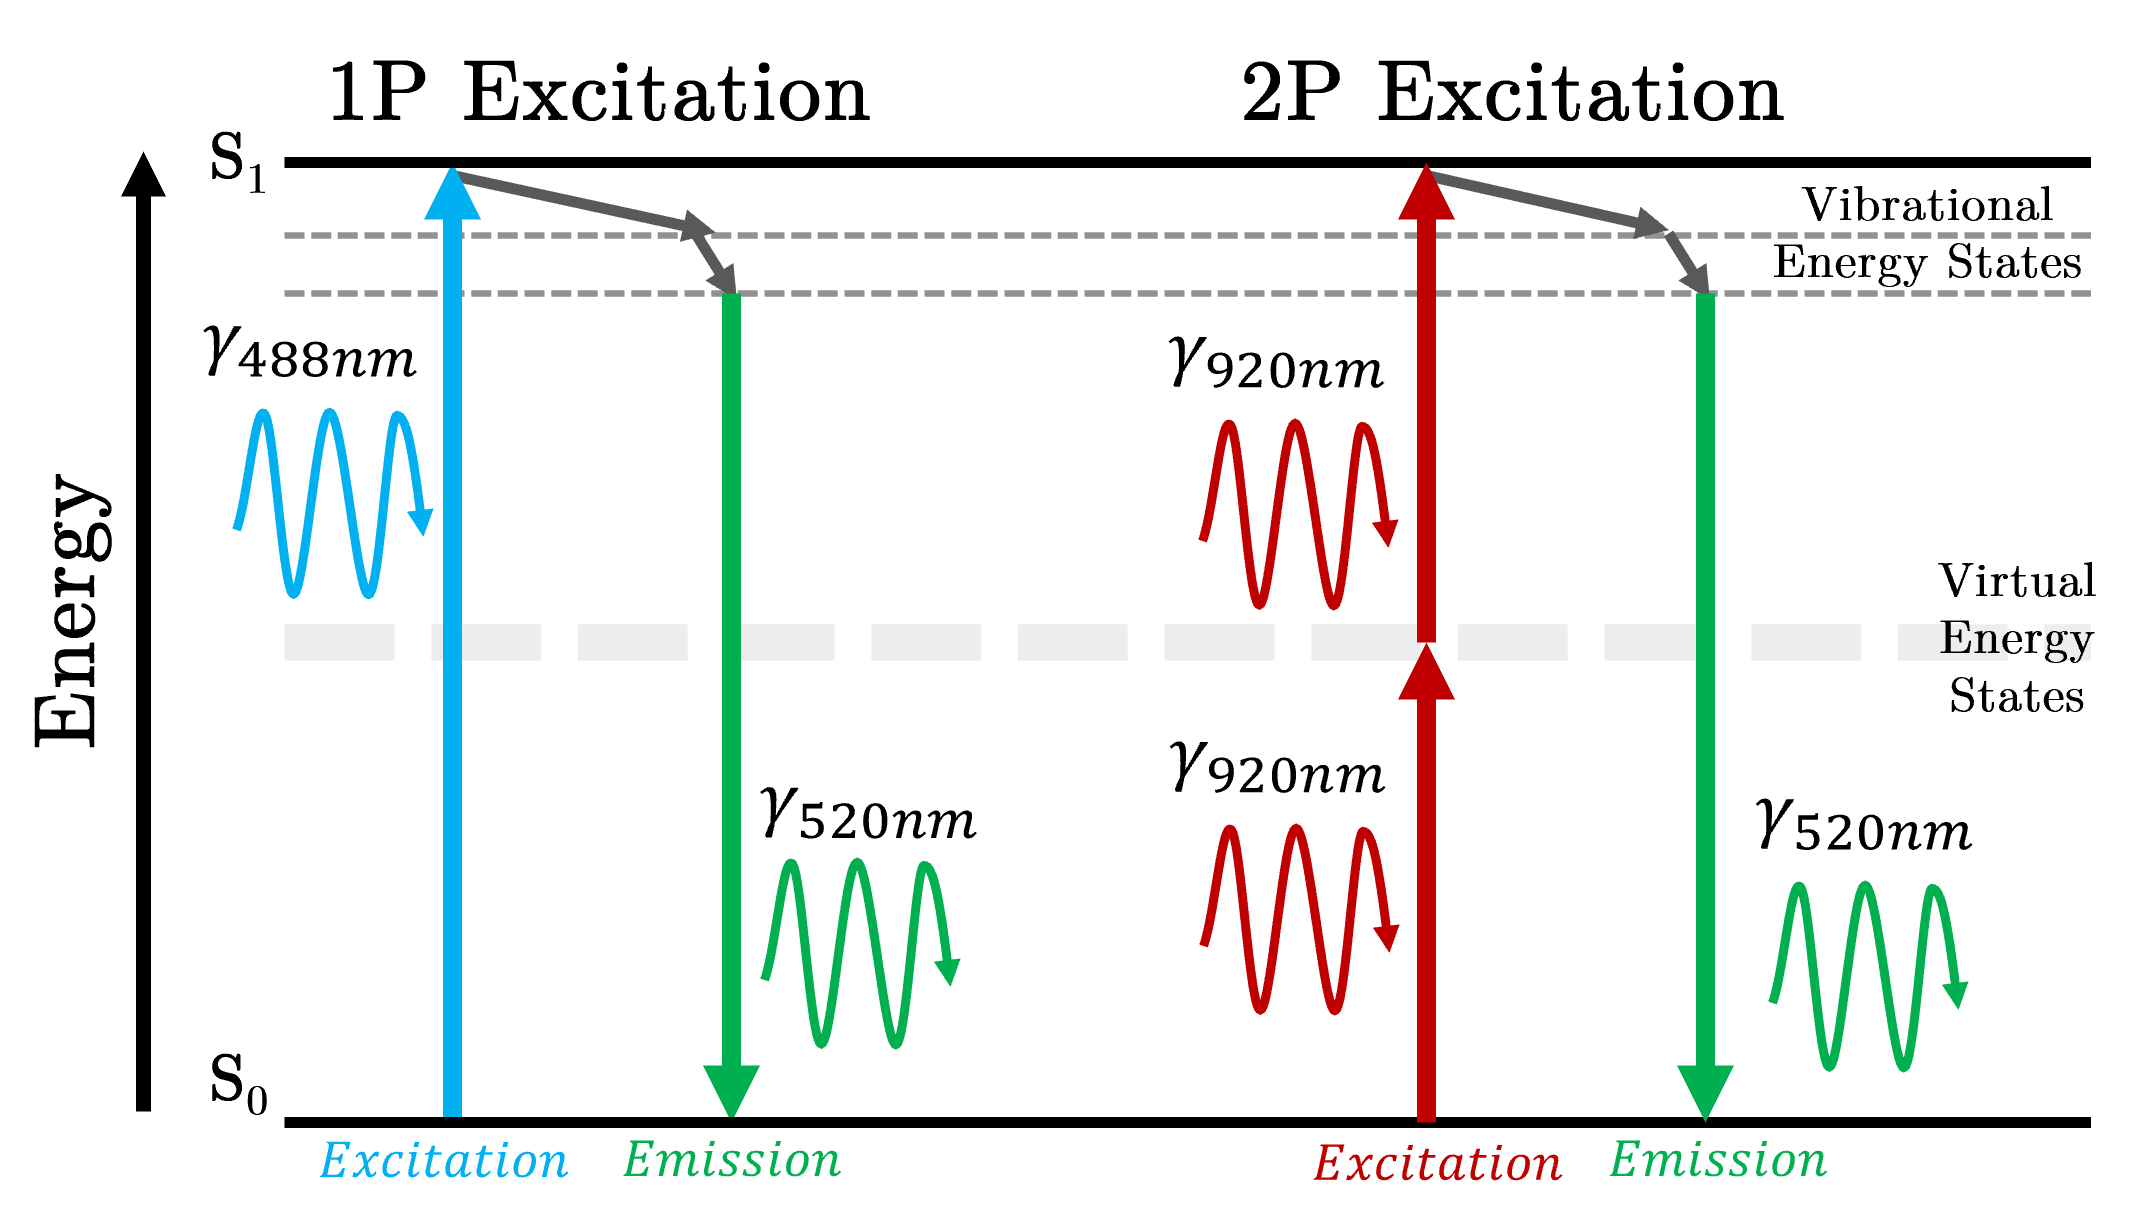
\includegraphics[width=0.9\linewidth]{Figures/Fluorescence.PNG}
\caption{\textbf{Jablonski Energy Diagram}}
\raggedright
1P and 2P fluorescence processes are shown in terms of energy exchange between input excitation photons (either one or two), a fluorescent molecule, and released emission photons. The key insight is the spectral difference between the light used to generate the increase in energy state and the emitted photon. 2P excitation is described in detail in Chapter 3.
\label{fig:fluorescence}
\end{figure*}



\chapter{1P Excitation Imaging in Neuroscience}
\section{Core 1P Microscopy Ideology}
The fluorescent physical process described in section one is the core operating principle of single photon (1P) imaging. In general, any single photon that is provided to the sample contains enough energy, on its own, to induce a fluorescence event. Such microscopy systems manifest typically in the form of a visible light source (usually a light emitting diode (LED), visible continuous wave laser, or arc-lamp), spectral filters and dichroic beamsplitters, focusing optics like an infinitely-conjugated objective assembly, a image forming tube lens, and an array detector such as a Complementary Metal-Oxide-Semiconductor (CMOS) image sensor. The majority of 1P microscopy systems can be decomposed into two main subsystems, one that generates appropriate photoexcitation into the sample, and one for collecting the fluorescent emission provided by the protein of interest. 

\subsection{Example 1P Microscope Setup and Operational Principles}
In the example of a 1P microscope used for GFP imaging, a visible, blue LED of $\approx$470nm wavelength would be collimated using a short focal length aspheric lens, then spectrally filtered with an excitation filter to remove frequency components outside of a desired pass-band. An excitation filter that is centered at 470 nm with a bandwidth of \textpm 20nm would be suitable for this purpose. The light would then pass through a simple lens  before being reflected on a dichroic mirror. This spectral beam splitter is critical to the operation of the microscope and serves to separate the excitation light (via reflectance) from the collected fluorescence (via transmission). As such, the dichroic requires specific consideration, and something on the scale of the T495lpxr from Chroma would work nicely. The excitation light will reflect off the dichroic mirror, then enter an infinitely conjugated objective assembly, with the simple lens having focused the light onto the rear pupil plane of the objective. In this configuration, the excitation light being emitted from the objective, into the brain, will intentionally not be focused to a single point, rather it will illuminate the entire focal plane in a wide-field manner. However, because each 470nm photon used for photoexcitation contains enough energy to locally generate a fluorescent event in any GFP molecule it experiences, there is a considerable amount of background fluorescence generated above and below the focal plane of interest. This additional fluorescence contributes background and limits resolution, especially in dense neuronal populations. The fluorescence that is generated will be collected over a fixed numerical aperture (NA) as defined by the objective lens. The equation for numerical aperture is as follows: 

\begin{equation}
NA = n \sin \theta
\end{equation}

\noindent where $n$ is the refractive index of the medium in which the lens is working, $\theta$ is the half-angle of the maximum cone of light that can enter or exit the lens. Once fluorescence is collected, it is transmitted through the dichroic mirror, before being further spectrally filtered with an emission filter. A filter centered at 520nm with a bandwidth of \textpm 20nm, or alternatively a longpass filter beyond 500nm would be suitable. Following spectral filtering, the light that came only via fluorescent emission is then focused by a tube lens to form an image onto an 2D image sensor. The optical resolution of a diffraction limited 1P imaging system depends strongly on numerical aperture, and scales as the following:


\begin{equation}
    R_{lateral(1P)} = \frac{\lambda}{2 \cdot \text{NA}}
\end{equation}

\begin{equation}
    R_{axial(1P)} = \frac{2 \cdot \lambda}{\text{NA}^2}
\end{equation}


\chapter{UCLA 2P Miniscope: Design Philosophy and Filling a Gap in the Field}

\section{A cost-effective 2P Miniature Microscope}
We developed the UCLA 2P Miniscope to be cost effective without significantly compromising performance. Our entire microscope headpiece can be built for less than \$7.5k USD currently with low production numbers and likely with scaling can be reduced to approximately \$5k USD each. The majority of the cost comes in the form of the custom optical assemblies which are assembled, coated, and tested individually by Optics Technology in New York, USA. With scale, we predict these assemblies to drop in cost and further lower barriers of entry to labs hoping to use miniature 2P microscopes to study neural dynamics in freely behaving animals. To our understanding, this is the first miniature 2P microscope that is open sourced and able to be built for less than \$10k USD. 

\begin{table}
    \centering
    \begin{tabular}{llccc}
      \textbf{Component}   & \textbf{Manufacturer} & \textbf{Quantity} & \textbf{Cost} & \textbf{Subtotal}\\
      \hline
      \\
        Objective Lens & OT, Custom - 1 & 1 & \$4000 & \$4000\\
        Tube Lens & OT, Custom - 2 & 1 & \$1100 & \$1100\\
        Scan Lens & ThorLabs, AC050-010-B & 2 & \$51 & \$102\\
        Aspheric Lens & Newport, KGA170-B & 1 & \$104 & \$104\\
        Collection Lens & Edmund, 47-895 & 1 & \$62 & \$62\\
        2P Dichroic & Chroma, ZT775sp-2p & 1 & \$540 & \$540\\
        1P Dichroic & Chroma, T550lpxr & 1 & \$112 & \$112\\
        2P Emission Filter & Chroma, ET750sp & 2 & \$150 & \$300\\
        MEMS Scanner & Mirrorcle, A7M20.2-2000AL & 1 & \$591 & \$591\\
        Electrotunable Lens & Varioptic, A-25H1 & 1 & \$135 & \$135\\
        Mechanical Housings & Custom Made & 4 & \$10 & \$40\\
        PCBs & PCBWay, Custom Made & 1 & \$50 & \$50\\
        SiPM Detectors & Hamamatsu, S13360-3075PE & 2 & \$52 & \$105\\
         &  &  &  & \ \textbf{\$7243}\\

    \end{tabular}
    \caption{\textbf{Cost breakdown for the UCLA 2P Miniscope microscope headpiece}}
    \raggedright
    These costs are as of March 2024 when components were purchased at small scale. Please note that these expenses do not include key additional hardware, such as laser and traditional 2P microscope acquisition electronics
    \label{tab:cost_table}
\end{table}



\section{Prioritization Given Towards Ease of Assembly}
Our goal is to make miniature 2P microscopy as accessible to as many users as possible, while pushing the technical limits of what such systems are capable of achieving. Intentional design tradeoffs were made throughout the engineering process which ultimately prioritized user adoption over absolute performance. One example of this is the tunable lens. Other microscope systems use stacks of piezoelectric tunable interfaces to generate sufficient optical power to translate the focal plane by respectable amounts. While these elements are extremely lightweight (0.06g) and seem to perform very well, they are difficult to align together into a colinear, stacked assembly and install into the microscope body, resulting in a barrier to entry for users. In contrast, we use off-the-shelf Varioptic lenses which are substantially heavier (0.36g) yet are easy to source and install. This intentional decision was made not due to performance, but to achieve increased user friendliness and adoption capability. We believe that these benefits outweigh the cost associated with the modest increase in weight of the UCLA 2P Miniscope compared to other similar systems. 

\section{Designed to Be Sensitive to Dim Signals}
The UCLA 2P miniscope also uses on-board Si-based detectors, similar to those used in 3P applications. Such a detection scheme substantially improves collection efficiency of the microscope and thus makes resolving dynamics from deep structures like DG possible, at the expense of added weight. The microscope in its current form uses two detectors, to record from red and green channels, as well as collection optics and spectral filters to isolate colors onto discrete detectors. Because of this, the microscope incurs some additional weight, at the benefit of being able to record deep and challenging brain areas in two colors. 


\section{Future Directions}
\subsection{Extending Current Technology}
The most straightforward approach to thinking about future developments within miniature microscopy is to begin with incremental improvements that come from the onset of new and innovative technology that have yet to make its way to the field. To my view, these include: new scanner technologies for autonomous vehicle applications, methods that utilize the new support of polarization maintenance in hollow-core photonic crystal fiber, integration with off-the-shelf freeform miniature lens assemblies and the utilization of diffractive optical elements (DOE). 
\\

\section{Conclusions}
Miniature microscopy is a critically important optical tool for neuroscientists studying neural circuit mechanisms that underly many naturalistic behaviors. Specifically, miniature microscopes allow for the study of cells involved in behaviors that cannot be replicated sufficiently within head-fixed contexts, like spatial navigation or social interaction. While these tools have immense power, the majority of miniature microscopes are single photon in nature, and thus, suffer from scattering and a lack of optical sectioning ability. As a result, 1P systems are only able to resolve somas that are within a few microns from either a cranial window or implanted GRIN lens. To overcome these limitations and study dynamics from deep cellular networks or fine cellular projections like dendrites and axons, multiphoton approaches are necessary. The open-source miniature 2P microscope presented here extends the capabilities of the UCLA Miniscope Project and enables the rest of the community to build and use the hardware and software described for minimal expense. The UCLA 2P Miniscope costs less than \$10k USD, has submicron resolution and optical sectioning abilities that make it able to address new scientific questions in freely behaving animals. We used it to resolve dendrites in freely behaving animals, as well as resolving dense, tightly packed granule cells hundreds of microns into tissue. Altogether, this innovative tool will contribute to scientific discoveries and further our understanding of how neural dynamics encode behavior in a number of experimental contexts. 


\bibliographystyle{UCLAthesis}
\bibliography{thesis}

\end{document}